\AtBeginDocument{\renewcommand{\bibname}{References}}
\documentclass[12pt]{report}
\usepackage[a4paper, margin=1in]{geometry}
\usepackage{graphicx}
\graphicspath{{assets}}
\usepackage[hidelinks]{hyperref}
\usepackage{cite}
\usepackage{float}
\usepackage{setspace}
\usepackage{parskip}
\usepackage{url}
\def\UrlBreaks{\do\/\do-}
\renewcommand{\arraystretch}{1.2}
\onehalfspacing
\setlength{\parindent}{15pt}

\begin{document}

\begin{titlepage}
	\setlength{\parskip}{0pt}
	\singlespacing
	\begin{center}
		
\includegraphics[width=0.4\linewidth]{aastu}

		\Large
		Addis Ababa Science and Technology University \\
		College of Engineering \\
		Department of Software Engineering

		\vspace*{1.5cm}

		\Huge
		\textbf{AI Powered E-Commerce Platform}

		\vspace{0.25cm}

		\LARGE
		Senior Capstone Research Project

		\vspace{1.25cm}

		\vfill
	\end{center}
\end{titlepage}

\begin{titlepage}
	\setlength{\parskip}{0pt}
	\singlespacing
	\begin{center}
		
\includegraphics[width=0.4\linewidth]{aastu}

		\Large
		Addis Ababa Science and Technology University \\
		College of Engineering \\
		Department of Software Engineering

		\vspace*{1cm}

		\LARGE
		\textbf{Title: AI Powered E-Commerce Platform}

		\vspace{0.25cm}

		\LARGE
		Senior Capstone Research Project

		\vspace{1.25cm}

		\Large
		\begin{tabular}{ |r|l|l| }
			\hline
			\multicolumn{3}{|c|}{\textbf{Group Members}} \\
			\hline
			No. & Name              & ID                 \\
			\hline
			1.  & Amanuel Ayana     & ETS 0110/13        \\
			2.  & Amanuel Dagnachew & ETS 0112/13        \\
			3.  & Amanuel Mandefro  & ETS 0121/13        \\
			4.  & Amanuel Solomon   & ETS 0126/13        \\
			5.  & Beamanuel Tesfaye & ETS 0180/13        \\
			\hline
		\end{tabular}


		\vfill

		\Large
		\begin{tabular}{@{}p{1in}p{3in}@{}}
			Advisor:   & \hrulefill \\
			Signature: & \hrulefill \\
		\end{tabular}

		\vspace{1.25cm}
		Section A\\
		January 2025
	\end{center}
\end{titlepage}
\newpage

\pagenumbering{roman}

\chapter*{Acknowledgment}
\addcontentsline{toc}{chapter}{\protect\numberline{}Acknowledgment}

Lorem  ipsum  dolor  sit  amet,  consectetuer  adipiscing
elit. Etiam  lobortisfacilisis sem.  Nullam nec mi et
neque pharetra sollicitudin.  Praesent imperdietmi nec ante.
Donec ullamcorper, felis non sodales...
\newpage

\tableofcontents

\listoffigures
\addcontentsline{toc}{chapter}{\protect\numberline{}List Of Figures}

\listoftables
\addcontentsline{toc}{chapter}{\protect\numberline{}List Of Tables}

\clearpage
\pagenumbering{arabic}

\newpage

\chapter{Introduction}
The rapid growth of e-commerce has fundamentally changed how businesses and consumers
interact. Online platforms offer unparalleled convenience and access to goods, yet they often
fail to address critical issues such as personalized user experiences, efficient product
discovery, and seamless transactions. These gaps lead to frustration for consumers and missed
opportunities for sellers.

The evolution of digital marketplaces over the past two decades has been driven by advances
in technology and changing consumer expectations. While early e-commerce platforms
primarily focused on listing and selling products, modern platforms must adapt to a more
dynamic and competitive environment. Consumers today demand intuitive interfaces,
personalized recommendations, and faster delivery options, forcing businesses to innovate or
risk obsolescence. Studies show that over 40\% of consumers abandon online purchases due to
poor navigation or inadequate product information.\cite{c1}\cite{c2}

Artificial intelligence (AI) and machine learning have emerged as transformative tools in
addressing these issues. By analyzing user behavior, preferences, and purchasing patterns,
AI-powered systems can deliver personalized experiences and enhance product discovery.
Leading platforms such as Amazon and Alibaba have demonstrated the effectiveness of these
technologies in increasing customer satisfaction and boosting sales \cite{c2}\cite{c3}. Despite these
advancements, many small to mid-sized businesses struggle to integrate such sophisticated
systems due to resource constraints, leaving a significant portion of the market underserved.
\cite{c3}

Recognizing these challenges, our app (\textbf{PRICO}) is envisioned as a next-generation
e-commerce platform powered by advanced artificial intelligence. With features like
personalized product recommendations, barcode-based tools for sellers and buyers, integrated
payment systems, and delivery services, our app (\textbf{PRICO}) aims to set a new benchmark in
the industry. By leveraging state-of-the-art technologies, our app (\textbf{PRICO}) not only enhances
the shopping experience but also empowers businesses to thrive in a competitive digital
marketplace. Moreover, our app (\textbf{PRICO}) seeks to bridge the gap for smaller enterprises,
enabling them to compete effectively with industry giants by providing accessible and
scalable solutions. \cite{c1}\cite{c4}

In an increasingly digitized world, platforms like our app (\textbf{PRICO}) represent the future of
commerce. By addressing the current limitations of e-commerce and focusing on innovation,
our app (\textbf{PRICO}) aims to redefine the relationship between buyers and sellers. Its
commitment to leveraging cutting-edge technologies ensures a seamless, efficient, and
satisfying experience for all stakeholders involved. \cite{c2}\cite{c5}

\section{Statement of the Problem}

In today's digital economy, e-commerce platforms have become essential for bridging the gap
between sellers and buyers. However, many existing platforms fail to address key challenges
such as personalized shopping experiences, efficient product discovery, and seamless
transactions. Consumers are often overwhelmed by excessive options, while sellers struggle
to reach their target audience effectively. These gaps highlight the need for a more intelligent
and user-centric platform that can transform the e-commerce experience.

For instance, platforms like Ashewa offer subscription-based packages such as yearly,
monthly, or semi-monthly. That allows vendors to sell products and access exclusive features.
While this model provides sellers with a marketplace, it may not sufficiently address issues
related to product discovery and personalized customer engagement. Without advanced
algorithms to tailor recommendations, consumers can become overwhelmed by the sheer
volume of options, leading to decision fatigue and abandoned shopping carts. Studies have
shown that the average online shopping cart abandonment rate worldwide is approximately
70\%.\cite{c6}

Similarly, platforms like Jiji.et allow anyone to post products with minimal oversight, which
has led to concerns about scams and security risks. The lack of stringent verification
processes for sellers can result in fraudulent listings, eroding consumer trust and deterring
potential buyers. In contrast, implementing a system that permits only verified vendors to sell
products can significantly enhance trust and safety in online transactions. Building trust with
customers is essential in driving more sales in any marketplace, especially in an online
marketplace where customers need reassurance that they can trust the sellers they are using. \cite{c7}

Moreover, the absence of integrated payment systems and reliable delivery services in some
platforms further complicates the transaction process. Consumers may face challenges in
completing purchases smoothly, and sellers might encounter difficulties in managing orders
and logistics. A comprehensive e-commerce solution that incorporates secure payment
gateways and efficient delivery mechanisms is crucial to meet the evolving demands of both
consumers and merchants.

Addressing these issues requires a holistic approach that combines advanced technology with
user-centric design. By focusing on personalized experiences, verified vendor systems, and
seamless transaction processes, the proposed platform aims to redefine the e-commerce
landscape, fostering a more trustworthy and efficient marketplace for all stakeholders.

\section{Objectives}

\subsection{General Objectives}

Our general objective is to develop an AI-powered e-commerce platform. With enhanced user
engagement through personalized product recommendations, efficient scanning features, and
reliable payment and delivery integrations.

\subsection{Specific Objectives}

\begin{enumerate}
	\item \textbf{Requirement Gathering}
	      \begin{itemize}
		      \item Identify and document key functional and non-functional requirements
		            of the platform, including user needs and business goals.
		      \item Analyze existing e-commerce systems like Ashewa and Jiji.et to
		            identify gaps and challenges to address.
	      \end{itemize}
	\item \textbf{System Design and Architecture}
	      \begin{itemize}
		      \item Design a user-friendly interface for both buyers and sellers, focusing
		            on ease of navigation and accessibility.
		      \item Develop a scalable and secure architecture to handle large volumes of
		            data and concurrent users.
		      \item Plan database structures to efficiently store and retrieve product and
		            user information.
	      \end{itemize}
	\item \textbf{AI-Based Recommendation Engine}
	      \begin{itemize}
		      \item Implement an AI-driven recommendation system to provide
		            personalized product suggestions based on user preferences and
		            browsing history.
		      \item Continuously update the recommendation model with real-time data to
		            improve accuracy and relevance.
	      \end{itemize}
	\item \textbf{Feature Development}
	      \begin{itemize}
		      \item Integrate "Scan to Post" functionality, allowing sellers to post products
		            by scanning barcodes, minimizing manual data entry.
		      \item Implement "Scan to Find" functionality for buyers, enabling quick and
		            precise product discovery.
		      \item Incorporate Chapa payment gateway to ensure secure and seamless
		            transactions.
		      \item Develop a robust delivery service module with real-time tracking to
		            enhance customer satisfaction.
	      \end{itemize}
	\item \textbf{Vendor Verification System}
	      \begin{itemize}
		      \item Design and implement a vendor verification mechanism to ensure only
		            legitimate and trustworthy sellers can list products on the platform.
		      \item Create an intuitive registration and verification process for vendors.
	      \end{itemize}
	\item \textbf{Scalability and Security Enhancements}
	      \begin{itemize}
		      \item Optimize the platform to support a growing user base and large-scale
		            operations.
		      \item Implement advanced security measures, including data encryption,
		            secure APIs, and fraud detection algorithms.
	      \end{itemize}
	\item \textbf{Testing and Quality Assurance}
	      \begin{itemize}
		      \item Conduct thorough unit testing to ensure all modules function as
		            expected.
		      \item Perform integration and system testing to validate the interoperability
		            of different components.
		      \item Test the platform under various load conditions to ensure scalability
		            and performance.
	      \end{itemize}
	\item \textbf{User Training and Documentation}
	      \begin{itemize}
		      \item Provide comprehensive user guides and documentation for both buyers
		            and sellers.
		      \item Conduct training sessions or create tutorials to familiarize users with
		            platform features.
	      \end{itemize}
	\item \textbf{Deployment}
	      \begin{itemize}
		      \item Deploy the platform on a reliable hosting service with appropriate
		            monitoring and maintenance tools.
		      \item Set up CI/CD pipelines to facilitate seamless updates and new feature
		            rollouts.
	      \end{itemize}
	\item \textbf{Post-Deployment Support and Maintenance}
	      \begin{itemize}
		      \item Monitor platform performance and user feedback after deployment to
		            identify and address any issues.
		      \item Regularly update the platform with new features and enhancements
		            based on user needs and technological advancements.
	      \end{itemize}
\end{enumerate}

\section{Scope and Limitations}

\subsection{Scope}

The scope of this study includes developing a functional prototype of our app (\textbf{PRICO}) that
incorporates AI-driven features, barcode scanning tools, Chapa payment integration, and
delivery services. While the project focuses on delivering core functionalities, it also aims to
enhance user engagement and experience by integrating innovative features and ensuring a
secure and scalable platform.

The project will cover the following key areas:

\begin{itemize}
	\item \textbf{AI-Driven Features}
	      \begin{itemize}
		      \item Implementation of an AI-based recommendation engine to provide
		            personalized product suggestions tailored to user preferences.
		      \item Continuous learning capabilities to improve recommendation accuracy over
		            time.
	      \end{itemize}
	\item \textbf{Verified Vendor System}
	      \begin{itemize}
		      \item Introduction of a vendor verification mechanism to ensure only legitimate
		            sellers can list products.
		      \item A focus on building trust and reducing risks of fraud and scams within the
		            platform.
	      \end{itemize}
	\item \textbf{Barcode Scanning Tools}
	      \begin{itemize}
		      \item Development of "Scan to Post" functionality for sellers, enabling effortless
		            product listings by scanning barcodes.
		      \item Implementation of "Scan to Find" functionality for buyers, allowing instant
		            and precise product searches using barcode scanning.
	      \end{itemize}
	\item \textbf{Chapa Payment Integration}
	      \begin{itemize}
		      \item Incorporation of Chapa payment gateway to facilitate secure and seamless
		            online transactions.
		      \item Support for multiple payment methods to enhance accessibility for users.
	      \end{itemize}
	\item \textbf{Delivery Services}
	      \begin{itemize}
		      \item Creation of a robust delivery system with real-time tracking to provide
		            transparency and reliability for users.
		      \item Development of delivery status notifications to keep buyers informed
		            throughout the process.
	      \end{itemize}
	\item \textbf{Reels-Like Video Feature}
	      \begin{itemize}
		      \item Integration of a reels-like video showcasing feature, enabling sellers to upload
		            short, engaging videos of their products.
		      \item Implementation of a scrolling video feed to provide buyers with an interactive
		            and immersive shopping experience.
		      \item AI-powered video analytics to highlight trending products and improve
		            discoverability.
	      \end{itemize}
\end{itemize}

This project emphasizes a user-centric approach by prioritizing features that address existing
gaps in the market, such as personalized experiences, secure transactions, and innovative
ways of showcasing products. The ultimate goal is to create a secure and scalable
e-commerce platform that delivers value to both buyers and sellers.

\subsection{Limitations}

[\textit{To be written on \textbf{Second Phase}\dots}]

\section{Methodology}

The development of our app (PRICO) will adopt the \textbf{Incremental Development Model},
which emphasizes building the application in manageable increments. This approach is ideal
for projects requiring iterative development and continuous feedback integration. By
delivering functional modules in stages, the team can incorporate user input early in the
development cycle, refine features iteratively, and ensure that the final system aligns with
user needs. \cite{c8}

\subsection{Requirement Gathering}

The requirement-gathering process will focus on understanding the needs of both buyers and
sellers in the e-commerce ecosystem. To achieve this, a \textbf{survey-based approach} will be
employed, supplemented by interviews with potential users. Surveys will allow the collection
of quantitative data from a larger audience, helping to identify trends and priorities.
Interviews will provide qualitative insights into specific pain points and desired features. This
mixed-method approach ensures a comprehensive understanding of user requirements.

This methodology was chosen because surveys enable scalable data collection, making it
possible to gather a diverse set of requirements within a limited timeframe.\cite{c9} Interviewing,
on the other hand, provides the depth needed to uncover nuanced user expectations that might
not emerge from surveys alone.

\subsection{Requirement Analysis}

The gathered requirements will be analyzed using Object-Oriented Analysis (OOA) and
Unified Modeling Language (UML). OOA is particularly effective for translating user
requirements into real-world scenarios by focusing on objects and their interactions within
the system.\cite{c10} UML diagrams, including use-case diagrams, class diagrams, and deployment
diagrams, will provide a structured and visual representation of these requirements, ensuring
clear communication among stakeholders.

\subsection{System Design}

The design phase will leverage \textbf{Figma} for UI/UX design, ensuring an intuitive and engaging
interface. Figma’s collaborative features make it suitable for a project involving multiple
contributors, enabling real-time feedback and iteration.\cite{c11} High-fidelity prototypes and
wireframes will be created to visualize the user journey and ensure alignment with the project
objectives.

\subsection{Implementation}

The implementation phase will follow the incremental model, developing key modules such
as the AI recommendation engine, barcode scanning features, Chapa payment integration,
and delivery tracking in separate iterations. This staged approach ensures that each module is
thoroughly developed and tested before integration into the larger system.

The architectural design of the system will adopt a \textbf{monolithic} structure with a few \textbf{external services} to enhance
scalability and maintainability. \textbf{Flutter} will be used for mobile application development due
to its cross-platform capabilities and support for a rich set of prebuilt UI components. \textbf{React}
will be employed for the web application, as it provides a modular and efficient way to build
dynamic user interfaces. \textbf{Go} will serve as the backend language, chosen for its
performance efficiency and concurrency management, which are essential for an e-commerce
platform expected to handle high traffic and transactions.

\subsection{Testing}

A combination of \textbf{unit testing} and \textbf{automated testing} will be employed to ensure the
reliability of the system. Unit tests will validate the functionality of individual components,
ensuring that each performs as expected. Automated testing tools, such as \textbf{Selenium} for the
web app and \textbf{Appium} for the mobile app, will be used to simulate user interactions and
identify issues early in the development cycle. For API testing we’re going to use \textbf{Postman}
or \textbf{Bruno}. These tools were selected for their ability to handle cross-platform testing
efficiently. \cite{c1201} \cite{c1202}

In addition to functional testing, performance testing will be conducted to evaluate the
system’s ability to handle concurrent users and transactions. Tools like \textbf{JMeter} will be
utilized for load testing, ensuring the platform’s scalability and resilience.

\subsection{Deployement}

The final prototype will be deployed using cloud-based solutions such as \textbf{Hahu Cloud},
\textbf{Yegara Host}, or \textbf{Telecloud} to provide a scalable and secure hosting environment. Containerization
tools like Docker will be used to streamline deployment and ensure consistency across
development, testing, and production environments.

\section{Plan of Activities}

\begin{enumerate}
	\item \textbf{Define Project Goals and Objectives (November)}
	      \begin{itemize}
		      \item Brainstorm project vision and goals.
		      \item Document initial objectives and scope.
		      \item Conduct stakeholder meetings for alignment.
	      \end{itemize}
	\item \textbf{Requirement Analysis and Design (December)}
	      \begin{itemize}
		      \item Gather requirements via surveys and interviews.
		      \item Analyze data using object-oriented methods.
		      \item Design system architecture using UML diagrams.
		      \item Create wireframes and prototypes using Figma.
	      \end{itemize}
	\item \textbf{System Architecture (January)}
	      \begin{itemize}
		      \item Design database schema.
		      \item Design monolithic core and define external services.
		      \item Choose development frameworks and tools.
	      \end{itemize}
	\item \textbf{Prototype Development (February)}
	      \begin{itemize}
		      \item Develop basic front-end with Flutter and React.
		      \item Create a backend API with Go.
		      \item Implement minimal viable features.
	      \end{itemize}
	\item \textbf{Integration of Features (March \& April)}
	      \begin{itemize}
		      \item Implement an AI-based recommendation system.
		      \item Add Chapa payment integration.
		      \item Develop barcode scanning tools.
		      \item Introduce reels-like video showcasing feature.
	      \end{itemize}
	\item \textbf{Testing and Debugging (April)}
	      \begin{itemize}
		      \item Conduct unit tests for individual components.
		      \item Perform automated system testing.
		      \item Perform user acceptance testing (UAT).
	      \end{itemize}
	\item \textbf{Final Deployment (April)}
	      \begin{itemize}
		      \item Deploy the system to the cloud.
		      \item Set up continuous integration and deployment (CI/CD).
	      \end{itemize}
	\item \textbf{Maintenance and Iterations (May)}
	      \begin{itemize}
		      \item Fix post-deployment bugs.
		      \item Improve system scalability and user experience.
		      \item Iterate on feedback from users.
	      \end{itemize}
	\item \textbf{Presentation and Defense (May)}
	      \begin{itemize}
		      \item Prepare a comprehensive project presentation.
		      \item Conduct a live demo of our app (\textbf{PRICO}).
		      \item Address questions during the defense.
	      \end{itemize}

\end{enumerate}

\begin{figure}[H]
	\begin{center}
		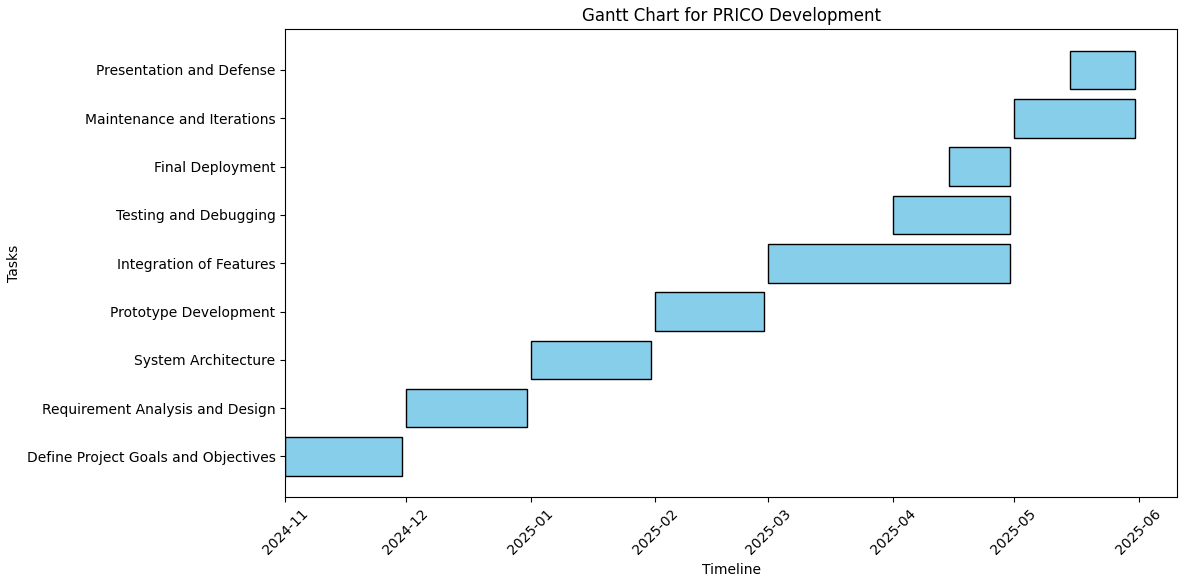
\includegraphics[width=0.95\textwidth]{images/gannt}
	\end{center}
	\caption{Gantt Chart for Plan Of Activities}
\end{figure}

\section{Budget Required}

\begin{table}[H]
	\begin{center}
		\begin{tabular}{|p{3cm}|p{5cm}|p{2.5cm}|p{2.5cm}||}
			\hline
			\textbf{Tool/Resource}               & \textbf{Purpose}                      & \textbf{Estimated Cost (USD)} & \textbf{Estimated Cost (ETB)} \\
			\hline
			Flutter SDK                          & Mobile App development framework      & Free                          & 0                             \\
			\hline
			React                                & Web app front-end development         & Free                          & 0                             \\
			\hline
			Go                                   & Backend Development                   & Free                          & 0                             \\
			\hline
			Figma                                & UI/UX design                          & Free (with education plan)    & 0                             \\
			\hline
			Firebase                             & Notifications                         & Free (Based on user base)     & 0 - 500                       \\
			\hline
			Chapa payment system                 & Payment gateway                       & Free                          & 0                             \\
			\hline
			Hosting Services                     & Cloud Deployment and Hosting          & See Table~\ref{tab:table2}    & See Table~\ref{tab:table2}    \\
			\hline
			Testing Tools (Postman, Bruno, etc.) & API \& unit testing                   & Free                          & 0                             \\
			\hline
			Transportation                       & For Requirement Gathering and Surveys & Fixed                         & 2000                          \\
			\hline
			\textbf{Total}                       &                                       &                               & 3300                          \\
			\hline
			\hline
		\end{tabular}
		\caption{Total Budget allocations}\label{tab:table1}
	\end{center}
\end{table}

\begin{table}[H]
	\begin{center}
		\begin{tabular}{|p{3cm}|p{3cm}|p{2.5cm}|p{2.5cm}||}
			\hline
			\textbf{Service}          & \textbf{Plan} & \textbf{Estimated Cost (USD)} & \textbf{Estimated Cost (ETB)} \\
			\hline
			Hahu Cloud                & Starter       & 4                             & 600                           \\
			\hline
			Yegara (Student Discount) & Mini Plan     & 6                             & 800                           \\
			\hline
			\hline
		\end{tabular}
		\caption{Budget allocations for Hosting Services}\label{tab:table2}
	\end{center}
\end{table}

\section{Feasibility Study}

\begin{enumerate}
	\item \textbf{Technical Feasibility}
	      \begin{itemize}
		      \item \textbf{Impact}: The project relies on modern technologies such as Flutter for mobile
		            development, React for the web app, and Go for backend development. All
		            these tools are well-documented, widely used, and compatible with the
		            project's requirements. Integration of Chapa payment and AI-based
		            recommendations can be achieved using existing APIs and libraries. However,
		            expertise in these tools and technologies is essential for timely delivery.
		      \item \textbf{Verdict}: Technically feasible, as the required tools and technologies are
		            accessible, and the team possesses the necessary skills.
	      \end{itemize}
	\item \textbf{Operational Feasibility}
	      \begin{itemize}
		      \item \textbf{Impact}: The system will improve e-commerce by addressing fraud, enhancing
		            user experience, and offering features like AI-based recommendations and
		            secure payment options. The operational requirements, such as vendor
		            verification and delivery tracking, align with the project goals and can be
		            implemented effectively with existing team capabilities.
		      \item \textbf{Verdict}: Operationally feasible, as the project objectives align with practical
		            implementation plans and user needs.
	      \end{itemize}
	\item \textbf{Economic Feasibility}
	      \begin{itemize}
		      \item \textbf{Impact}: The estimated costs include development tools, hosting, and
		            operational expenses such as transportation for requirement gathering. With an
		            expected budget of $\sim$4,000 ETB (including transportation and hosting fees),
		            the project is affordable for the team. Potential revenue from vendors and
		            commissions will offset the initial investment.
		      \item \textbf{Verdict}: Economically feasible, as the budget is manageable, and the project
		            has potential for sustainable financial returns.
	      \end{itemize}
	\item \textbf{Legal Feasibility}
	      \begin{itemize}
		      \item \textbf{Impact}: Legal considerations include compliance with data protection
		            regulations, payment gateway agreements, and e-commerce laws in Ethiopia.
		            The use of Chapa payment requires adherence to financial transaction
		            standards. Vendor verification processes must comply with privacy and
		            consumer protection laws.
		      \item \textbf{Verdict}: Legally feasible, provided all regulatory and compliance
		            requirements are met.
	      \end{itemize}
	\item \textbf{Time Feasibility}
	      \begin{itemize}
		      \item \textbf{Impact}: The project timeline spans approximately six months, from
		            requirement gathering to deployment and maintenance. By following the
		            incremental approach, tasks can be broken into manageable sprints, allowing
		            for simultaneous development and testing. Delays in any phase, such as
		            integrating AI or payment systems, could affect the schedule.
		      \item \textbf{Verdict}: Time feasible, with a realistic timeline and proper project
		            management.
	      \end{itemize}
	\item \textbf{Environmental Feasibility}
	      \begin{itemize}
		      \item \textbf{Impact}: The project has a minimal environmental footprint, as it primarily
		            involves software development and cloud-based deployment. However,
		            ensuring energy-efficient hosting and promoting digital receipts over printed
		            materials could further reduce environmental impact.
		      \item \textbf{Verdict}: Environmentally feasible, with negligible negative impact.
	      \end{itemize}
	\item \textbf{Social Feasibility}
	      \begin{itemize}
		      \item \textbf{Impact}: The project promotes trust and security in e-commerce, addressing
		            common challenges like fraud and lack of vendor accountability. By
		            supporting local vendors and providing a user-friendly platform, it has a
		            positive social impact. However, educating users about the new system might
		            require additional effort.
		      \item \textbf{Verdict}: Socially feasible, with significant positive impact on local
		            e-commerce dynamics.
	      \end{itemize}
\end{enumerate}

\subsection*{Final Verdict}

The feasibility study indicates that \textbf{PRICO} is feasible in all evaluated dimensions. The
project is technically sound, operationally viable, economically manageable, legally
compliant, timely, environmentally sustainable, and socially impactful. With proper planning
and execution, \textbf{PRICO} is positioned to succeed.

\section{Significance of the Study}

Our app (\textbf{PRICO}) aims to redefine the e-commerce landscape by addressing critical
shortcomings in existing systems. Current platforms often lack robust fraud prevention
measures, personalized recommendations, and streamlined payment and delivery systems,
leaving users dissatisfied and vulnerable to scams. By integrating AI-powered features such
as tailored product recommendations, secure Chapa payment systems, and vendor
verification, our app (\textbf{PRICO}) ensures a user-friendly, secure, and efficient shopping
experience. The recent State of AI report published by McKinsey, 79\% of respondents stated
that integrating AI into marketing and sales has increased business revenue.\cite{c13}

For sellers, our app (\textbf{PRICO}) offers an optimized platform to showcase their products,
providing tools such as “Scan to Post” and reels-like video showcases to enhance product
visibility. These features empower local businesses to expand their reach, driving economic
growth and fostering digital transformation. Studies have shown that digital platforms can
significantly boost small and medium enterprises (SMEs) by reducing operational costs and
increasing market access by over 45\%. \cite{c14}

Moreover, our app (\textbf{PRICO}) addresses a gap in the Ethiopian e-commerce market by
creating a secure environment where only verified vendors can sell products, reducing scams
and fostering consumer trust. Trust is a critical factor in online marketplaces, as platforms
with higher trust levels have been found to generate 70\% more sales on average. \cite{c15} By
bridging these gaps, our app (\textbf{PRICO}) not only improves the online shopping experience but
also contributes to the broader economic and technological development of the region.

\section{Outline of the Study}

This study is organized into seven chapters, each addressing a specific aspect of the project to
provide a comprehensive overview of the development and evaluation of our app (\textbf{PRICO}).

\subsection*{Chapter 1: Introduction}

This chapter lays the foundation of the study, presenting the project background, objectives,
significance, and scope. It also discusses the methodologies employed throughout the
development process, highlighting the incremental approach to ensure adaptability and
iterative progress.

\subsection*{Chapter 2: Literature Review}

This chapter explores existing works in the field of e-commerce platforms, focusing on their
strengths, limitations, and the gaps they leave unaddressed. Comparative analysis identifies
areas where our app (\textbf{PRICO}) can introduce innovation, with a focus on AI integration,
vendor verification, and enhanced user experience.

\subsection*{Chapter 3: Problem Analysis and Modeling}

Chapter Three delves into the challenges faced by current e-commerce platforms, including
security risks, poor user personalization, and limited scalability. It presents a comprehensive
problem analysis and develops system models using UML diagrams and object-oriented
analysis to conceptualize our app (\textbf{PRICO})’s functionality.

\subsection*{Chapter 4: System Design and Architecture}

This chapter details the design and architecture of our app (\textbf{PRICO}), including UI/UX
prototypes created in Figma and system components like the AI recommendation engine,
barcode tools, and Chapa payment integration. It outlines the architectural framework and
highlights the technologies chosen for development.

\subsection*{Chapter 5: Implementation}

Chapter Five describes the step-by-step implementation of our app (\textbf{PRICO}), discussing
tools like Flutter for the mobile application, React for the web platform, and Go for backend
development. The chapter also addresses challenges encountered during the development
process and strategies used to overcome them.

\subsection*{Chapter 6: Testing and Evaluation}

This chapter evaluates the system’s performance and reliability through rigorous testing,
including unit and automated testing methods. Metrics such as response time, accuracy of AI
recommendations, and system security are analyzed to validate the project’s success in
meeting its objectives.

\subsection*{Chapter 7: Conclusion and Recommendations}

The final chapter summarizes the findings of the study, emphasizing the contributions of our
app (\textbf{PRICO}) to the e-commerce sector. It discusses the implications of the system, its
potential for scalability, and recommendations for future improvements and research
directions.

This structure ensures a logical flow, enabling the reader to understand the project from
conception to implementation and evaluation.

\chapter{Literature Review}

A comprehensive review of literature is integral to the foundation of any advanced research
endeavor, serving not only to contextualize the study but also to identify existing gaps and
chart a path forward. This chapter undertakes a critical examination of existing research
pertinent to the e-commerce domain, with an emphasis on the transformative role of artificial
intelligence(AI) and its applications. By systematically analyzing prior studies, the limitations
of existing systems, and the methodologies employed to overcome challenges, this chapter
positions our app (\textbf{PRICO}) as a timely and necessary intervention in Ethiopia’s evolving
digital economy. Furthermore, this literature review elucidates the interplay between global
trends and local peculiarities, emphasizing the need for innovative, scalable, and localized
solutions that address both technical and socio-economic barriers. By expanding upon these
themes, the review also demonstrates how our app (\textbf{PRICO}) can serve as a model for similar
interventions in other emerging markets.

\section{Study Related Works}

The proliferation of e-commerce platforms has catalyzed research into optimizing user
experiences, improving operational efficiency, and enhancing scalability. These studies span
diverse methodologies, applications, and contexts, offering valuable insights into the
challenges and opportunities within the field. Below is an expanded discussion of key works
that inform our app (\textbf{PRICO})’s development, focusing on their objectives, methodologies,
results, and broader implications.

\subsection*{AI for Personalized Recommendations}

Smith et al. tackled a persistent issue in e-commerce: the inadequacy of generic product
recommendations that fail to align with user preferences. \cite{c16} This misalignment often results
in reduced user engagement, lower conversion rates, and diminished platform loyalty. To
address these challenges, the researchers implemented a dual-layered approach combining
collaborative filtering and deep learning algorithms. Their study leveraged a dataset
comprising over one million user interactions, with the models trained to dynamically predict
user preferences based on behavior patterns, historical purchases, and demographic insights.

The findings were groundbreaking. The implementation of personalized recommendation
systems led to a 30\% increase in purchase rates, a 15\% reduction in customer churn, and a
significant improvement in session durations. These results underscore the transformative
potential of AI in enhancing user satisfaction and driving vendor visibility. Furthermore, the
study demonstrated that the deep learning layer was particularly effective in handling sparse
data scenarios, a common challenge in new or niche platforms. Smith et al. concluded by
emphasizing the scalability of such systems and advocating for their integration into
platforms seeking to sustain user engagement and optimize profitability. However, they also
highlighted the computational resource demands of deep learning models as a limitation,
particularly for resource-constrained markets where affordability and accessibility are critical
concerns. \cite{c16}

\subsection*{Barcode and QR Code Scanning in Retail}

Jones et al. investigated inefficiencies in product listing and discovered two critical
components of e-commerce operations. \cite{c17} Their study introduced a prototype system that
utilized barcode and QR code scanning to automate these processes. Sellers, for instance,
could scan product barcodes to auto-populate listing details, while buyers could retrieve
comprehensive product information by scanning codes. These features were particularly
targeted at enhancing the usability and efficiency of e-commerce platforms for both
small-scale vendors and consumers.

The methodology involved deploying a mobile application prototype in a controlled retail
environment with 50 sellers and 100 buyers. The results were striking: a 40\% reduction in
manual entry errors, a 25\% enhancement in buyer satisfaction, and a significant reduction in
the time sellers spent listing products. Moreover, the automation streamlined inventory
management, making it particularly beneficial for sellers managing large inventories. The
study’s broader implications extend to markets like Ethiopia, where manual workflows
dominate and human errors are prevalent. Jones et al. recommended widespread adoption of
such technologies to reduce human error, improve operational efficiency, and enhance user
satisfaction. However, they cautioned that the success of these systems hinges on widespread
access to scanning-compatible devices and robust mobile internet infrastructure factors that
remain significant barriers in under-resourced regions. \cite{c17}

\subsection*{AI in Payment and Delivery Systems}

Lee et al. focused on the persistent challenges of delayed transactions and inefficient logistics
in e-commerce \cite{c18}. Their study proposed an AI-driven framework that integrated payment
gateway optimization with dynamic delivery route adjustments. The payment model utilized
machine learning to recommend the most efficient payment options for users, factoring in
historical success rates, transaction speeds, and user preferences. Simultaneously, the delivery
system employed AI to adjust routes dynamically, considering real-time traffic conditions,
package distribution densities, and customer locations.

When implemented on a mid-sized e-commerce platform, the framework yielded a 20\%
reduction in transaction processing times and a 15\% improvement in delivery efficiency. The
study also reported a 10\% increase in customer retention, attributed to improved reliability
and user perception of platform efficiency. Beyond these metrics, the study explored the
scalability of such systems, noting their ability to integrate seamlessly with third-party
logistics providers. Lee et al. concluded that integrating AI into payment and delivery
workflows could significantly enhance overall system performance. Nonetheless, they
emphasized the need for robust data infrastructure to support such integrations, a challenge in
regions with limited technological penetration. The authors also recommended further
exploration of blockchain-based payment solutions to enhance security and transparency in
e-commerce transactions. \cite{c18}

\subsection*{Short-Form Video Promotion for E-Commerce}

Inspired by the success of platforms like TikTok, research into short-form video content as a
promotional tool has gained momentum. Chen et al. examined the impact of integrating
short-form video systems into e-commerce platforms to enhance product visibility and user
engagement \cite{c19}. Their study identified a common problem in traditional marketing
approaches: static product listings often fail to capture user interest in competitive online
spaces. To address this, they developed a system where vendors could upload 15–60 second
videos showcasing their products. The videos were designed to autoplay in a swipe-based
interface, allowing users to transition seamlessly between products.

The results were remarkable. Engagement rates increased by 50\%, with users spending
significantly more time interacting with the platform. Vendors reported a 35\% rise in
conversion rates, particularly for visually appealing or demonstrative products. Additionally,
the study highlighted the versatility of short-form videos in addressing diverse user
preferences, from showcasing detailed product specifications to creating emotionally
engaging narratives. Chen et al. recommended the integration of such systems for platforms
seeking to diversify user interaction models and capitalize on emerging trends in content
consumption. Challenges noted included the need for robust video compression and
streaming capabilities to ensure smooth playback in regions with limited bandwidth,
alongside considerations for user-generated content moderation to maintain platform quality. \cite{c19}

\subsection*{International and Local Systems}
\begin{itemize}
	\item \textbf{Amazon}: As a global leader, Amazon exemplifies the effective deployment of AI in
	      e-commerce. Its recommendation algorithms, logistics optimization, and payment
	      security systems set benchmarks for innovation. However, Amazon’s reliance on
	      high-resource infrastructure limits its applicability in developing regions, where
	      computational and operational resources are constrained. \cite{c16}
	\item \textbf{Jumia}: Jumia’s cash-on-delivery model highlights an effective adaptation to local
	      market dynamics across Africa. Despite this, its limited automation and reliance on
	      manual logistics processes constrain scalability and efficiency. \cite{c18}
	\item \textbf{Alibaba}: Renowned for empowering small and medium enterprises, Alibaba’s
	      platforms integrate sophisticated seller tools, including inventory management and
	      logistics optimization. However, the technical complexity of these systems presents
	      barriers to adoption in less technologically advanced contexts \cite{c17}.
	\item \textbf{Zmall}: Zmall’s emphasis on delivery services and tracking makes it unique among
	      Ethiopian platforms, but its lack of advanced discovery tools and personalization
	      features diminishes its competitiveness.
\end{itemize}

These systems collectively highlight the gap between the sophisticated capabilities of global
platforms and the foundational nature of local offerings. This disparity underscores the need
for our app (\textbf{PRICO})’s tailored, scalable, and AI-integrated approach.

\section{Identifying Milestones of the Related Literature and Finding the Gaps}

\subsection*{Milestones}

\begin{enumerate}
	\item \textbf{Personalized Recommendations}: The widespread adoption of AI-driven
	      recommendation systems, particularly by Amazon, has demonstrated their efficacy in
	      driving user engagement and boosting sales. These systems, however, remain
	      resource-intensive. \cite{c16}
	\item \textbf{Localized Payment Solutions}: Jumia’s cash-on-delivery approach illustrates the
	      necessity of aligning payment models with local user preferences, particularly in
	      cash-dependent economies. \cite{c18}
	\item \textbf{Mobile-First Adaptations}: Platforms like AliExpress have optimized for mobile
	      users, broadening access and improving usability. \cite{c17}
	\item \textbf{Trust Mechanisms}: Seller verification processes in platforms like Alibaba
	      underscore the importance of building trust, though their implementation in smaller
	      markets remains limited. \cite{c16}
	\item \textbf{Short-Form Video Integration}: Emerging platforms have demonstrated the efficacy
	      of short-form video in driving engagement, particularly for showcasing products in a
	      visually dynamic manner. \cite{c19}
\end{enumerate}

\subsection*{Gaps}

\begin{itemize}
	\item \textbf{Limited Personalization}: Ethiopian platforms lack the AI-driven capabilities needed
	      to enhance user engagement.
	\item \textbf{Scalability Issues}: Current systems struggle to accommodate growing user bases due
	      to reliance on manual processes.
	\item \textbf{Fragmented Systems}: Payment, delivery, and discovery functionalities often operate
	      in silos, reducing overall efficiency.
	\item \textbf{Weak Trust Mechanisms}: Inadequate verification processes and the absence of
	      refund policies undermine user confidence.
	\item \textbf{Lack of Modern Content Formats}: The absence of interactive content models, such
	      as short-form videos, limits user engagement and product visibility.
\end{itemize}

Our app (\textbf{PRICO}) is designed to address these gaps by delivering an integrated, AI-enhanced
platform that bridges the divide between global standards and local requirements.

\section{Lessons Learned from Literature}

The insights derived from the literature offer invaluable guidance for our app (\textbf{PRICO})’s
development:

\begin{enumerate}

	\item \textbf{Personalization as a Cornerstone}: AI-driven recommendation systems are pivotal in
	      enhancing user engagement and vendor visibility.
	\item \textbf{Localization as a Necessity}: Context-specific features, such as Telebirr integration,
	      ensure relevance and adoption in Ethiopia’s unique market.
	\item \textbf{Trust as a Foundation}: Verified sellers and secure payment systems are critical for
	      fostering confidence and driving platform adoption.
	\item \textbf{Automation for Efficiency}: Streamlined workflows, such as barcode scanning and
	      dynamic delivery routing, reduce inefficiencies and enable scalability.
	\item \textbf{Innovative Content Formats}: Short-form video systems offer a dynamic method to
	      showcase products, capturing user attention and driving conversions. \cite{c19}

\end{enumerate}

By synthesizing these lessons, our app (\textbf{PRICO}) aims to redefine e-commerce in Ethiopia,
offering a comprehensive and scalable solution that addresses existing challenges while
leveraging global best practices. The subsequent chapter will detail the problem analysis and
modeling processes that inform our app (\textbf{PRICO})’s architecture and implementation
strategies.

\chapter{Problem Analysis and Modeling}

\newpage

\nocite{*}
\bibliographystyle{src/IEEEtran}
\bibliography{src/references}
\addcontentsline{toc}{chapter}{\protect\numberline{}References}

\end{document}
